\documentclass[semifinal]{cpecmu}

%% This is a sample document demonstrating how to use the CPECMU
%% project template. If you are having trouble, see "cpecmu.pdf" for
%% documentation.

\projectNo{P069-1}
\acadyear{2021}

\titleTH{แอพพลิเคชั่นตั้งค่าและตรวจสอบอุปกรณ์เครือข่ายอัตโนมัติโดยใช้แอนสิเบิล}
\titleEN{Automation Application for Network Device Configuration and Verification with Ansible}

\author{นายชลนันต์ ทองไทย}{Chonlanan Thongthai}{640610625}
\author{นายทัตพงศ์ เสริมสุข}{Tadphong Sermsook}{640610636}
\author{นายศุภณัฐ วังทิพย์}{Suphanath Wangtip}{640612098}

\cpeadvisor{yuthapong}
\cpecommittee{dome}
\cpecommittee{pruet}

%% Some possible packages to include:
\usepackage[final]{graphicx} % for including graphics

%% Add bookmarks and hyperlinks in the document.
\PassOptionsToPackage{hyphens}{url}
\usepackage[colorlinks=true,allcolors=Blue4,citecolor=red,linktoc=all]{hyperref}
\def\UrlLeft#1\UrlRight{$#1$}

%% Needed just by this example, but maybe not by most reports
\usepackage{afterpage} % for outputting
\usepackage{pdflscape} % for landscape figures and tables. 

%% Some other useful packages. Look these up to find out how to use
%% them.
% \usepackage{natbib}    % for author-year citation styles
% \usepackage{txfonts}
% \usepackage{appendix}  % for appendices on a per-chapter basis
% \usepackage{xtab}      % for tables that go over multiple pages
% \usepackage{subfigure} % for subfigures within a figure
% \usepackage{pstricks,pdftricks} % for access to special PostScript and PDF commands
% \usepackage{nomencl}   % if you have a list of abbreviations

%% if you're having problems with overfull boxes, you may need to increase
%% the tolerance to 9999
% \tolerance=9999

\bibliographystyle{plain}
% \bibliographystyle{IEEEbib}

% \renewcommand{\topfraction}{0.85}
% \renewcommand{\textfraction}{0.1}
% \renewcommand{\floatpagefraction}{0.75}

%% Example for glossary entry
%% Need to use glossary option
%% See glossaries package for complete documentation.
\ifglossary
  \newglossaryentry{lorem ipsum}{
    name=lorem ipsum,
    description={derived from Latin dolorem ipsum, translated as ``pain itself''}
  }
\fi

%% Uncomment this command to preview only specified LaTeX file(s)
%% imported with \include command below.
%% Any other file imported via \include but not specified here will not
%% be previewed.
%% Useful if your report is large, as you might not want to build
%% the entire file when editing a certain part of your report.
% \includeonly{chapters/intro,chapters/background}

\begin{document}
\maketitle
\makesignature

\ifproject
\begin{abstractTH}
\hspace{0.5in}โครงงานนี้มีวัตถุประสงค์เพื่อพัฒนา Web Application ที่มีระบบอัตโนมัติสำหรับการตั้งค่าอุปกรณ์เครือข่ายและมีระบบที่สามารถตรวจสอบการทำงานของอุปกรณ์เครือข่ายว่าสิ่งที่ผู้ใช้ทำการตั้งค่าเข้าไปนั้นถูกต้องหรือไม่ และต้องการช่วยอำนวยความสะดวกให้ผู้ใช้สามารถตั้งค่าอุปกรณ์เครือข่ายได้ง่ายมากขึ้นและใช้ระยะเวลาในขั้นตอนการตั้งค่าอุปกรณ์เครือข่ายน้อยลง ซึ่งหากไม่มีระบบอัตโนมัติผู้ใช้ต้องทำการตั้งค่าอุปกรณ์เครือข่ายด้วยตัวเองและอาจทำให้เกิดความผิดพลาดและเสียเวลาโดยใช่เหตุได้
\end{abstractTH}

\begin{abstract}
    \hspace{0.5in}This project aims to develop a Web Application with an automated system for configuring network devices and a system for verifying the correctness of the configured settings. It aims to facilitate users in configuring network devices more easily and reducing the time spent on the configuration process. Without an automated system, users would have to manually configure network devices, which could lead to errors and wasted time.
\end{abstract}

\iffalse
\begin{dedication}
This document is dedicated to all Chiang Mai University students.

Dedication page is optional.
\end{dedication}
\fi % \iffalse

\fi % \ifproject

\contentspage

\ifproject
\figurelistpage

\fi % \ifproject

% \abbrlist % this page is optional

% \symlist % this page is optional

% \preface % this section is optional


\pagestyle{empty}\cleardoublepage
\normalspacing \setcounter{page}{1} \pagenumbering{arabic} \pagestyle{cpecmu}

\chapter{\ifenglish Introduction\else บทนำ\fi}

\section{\ifenglish Project rationale\else ที่มาของโครงงาน\fi}

\section{\ifenglish Objectives\else วัตถุประสงค์ของโครงงาน\fi}
\begin{enumerate}
    \item
\end{enumerate}

\section{\ifenglish Project scope\else ขอบเขตของโครงงาน\fi}

\subsection{\ifenglish Hardware scope\else ขอบเขตด้านฮาร์ดแวร์\fi}

\subsection{\ifenglish Software scope\else ขอบเขตด้านซอฟต์แวร์\fi}

\section{\ifenglish Expected outcomes\else ประโยชน์ที่ได้รับ\fi}

\section{\ifenglish Technology and tools\else เทคโนโลยีและเครื่องมือที่ใช้\fi}

\subsection{\ifenglish Hardware technology\else เทคโนโลยีด้านฮาร์ดแวร์\fi}

\subsection{\ifenglish Software technology\else เทคโนโลยีด้านซอฟต์แวร์\fi}

\section{\ifenglish Project plan\else แผนการดำเนินงาน\fi}

\begin{plan}{11}{2023}{2}{2024}
    \planitem{11}{2023}{11}{2023}{ศึกษาชุดคำสั่งการตั้งค่าและการตรวจสอบของ Cisco}
    \planitem{12}{2023}{1}{2024}{ศึกษาและทดลองใช้งาน Ansible}
    \planitem{1}{2024}{2}{2024}{ศึกษาและทดลองใช้งาน Ansible AWX}
    \planitem{2}{2024}{2}{2024}{เขียนรายงาน}
\end{plan}

\section{\ifenglish Roles and responsibilities\else บทบาทและความรับผิดชอบ\fi}
อธิบายว่าในการทำงาน นศ. มีการกำหนดบทบาทและแบ่งหน้าที่งานอย่างไรในการทำงาน จำเป็นต้องใช้ความรู้ใดในการทำงานบ้าง

\section{\ifenglish%
Impacts of this project on society, health, safety, legal, and cultural issues
\else%
ผลกระทบด้านสังคม สุขภาพ ความปลอดภัย กฎหมาย และวัฒนธรรม
\fi}

แนวทางและโยชน์ในการประยุกต์ใช้งานโครงงานกับงานในด้านอื่นๆ รวมถึงผลกระทบในด้านสังคมและสิ่งแวดล้อมจากการใช้ความรู้ทางวิศวกรรมที่ได้

\newcommand{\exinventory}{
  mail.example.com\\

  [webservers] \\
  foo.example.com \\
  bar.example.com \\
  
  [dbservers] \\
  one.example.com \\
  two.example.com \\
  three.example.com}

\chapter{\ifenglish Background Knowledge and Theory\else ทฤษฎีที่เกี่ยวข้อง\fi}

\section{Ansible}
\hspace{0.5in} Ansible คือ Open Source Software ที่ทำหน้าที่เป็นเครื่องมือสำหรับการจัดการระบบ (IT automation) ที่ใช้เพื่อควบคุมและจัดการระบบต่างๆ บนเครือข่าย ใช้งานง่าย มีประสิทธิภาพ และมีความยืดหยุ่นสูง เขียนด้วยภาษา python และใช้ SSH (Secure Shell) ในการเชื่อมต่อกับระบบต่างๆ Ansible ทำงานโดยใช้ Playbook ซึ่งเป็นไฟล์ YAML (Yet Another Markup Language) ที่กำหนดชุดของ tasks ที่จะรันบนระบบปลายทาง \\
รูปที่ \ref{fig:ansible_works} แสดงวิธีการทำงานของ Ansible

\begin{figure}[h]
  \begin{center}
    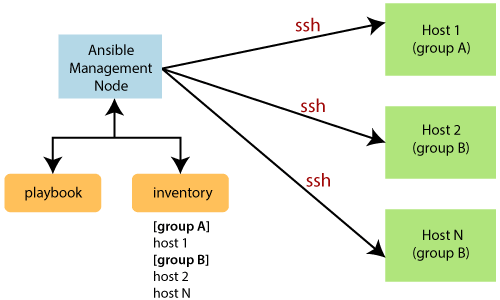
\includegraphics[scale=0.55]{ansible-works.png}
  \end{center}
  \caption[วิธีการทำงานของ Ansible]{วิธีการทำงานของ Ansible}
  \label{fig:ansible_works}
\end{figure}

\subsection{Inventory}
\hspace{0.5in} ไฟล์ที่ระบุรายการระบบปลายทางที่จะจัดการ \\
รูปที่ \ref{fig:inventory.ini} แสดงการเขียนไฟล์ Inventory.ini

\begin{figure}[h]
  \centering
  \fbox{
     \parbox{.6\textwidth}{\exinventory}
  }
  \caption[การเขียนไฟล์ Inventory.ini]{การเขียนไฟล์ Inventory.ini}
  \label{fig:inventory.ini}
\end{figure}

\subsection{Playbook}
\hspace{0.5in} ไฟล์ YAML ที่กำหนดชุดของ tasks ที่จะรันบนระบบปลายทาง \\
รูปที่ \ref{fig:ansible_playbook} แสดงการเขียน Playbook

\begin{figure}[h]
  \begin{center}
    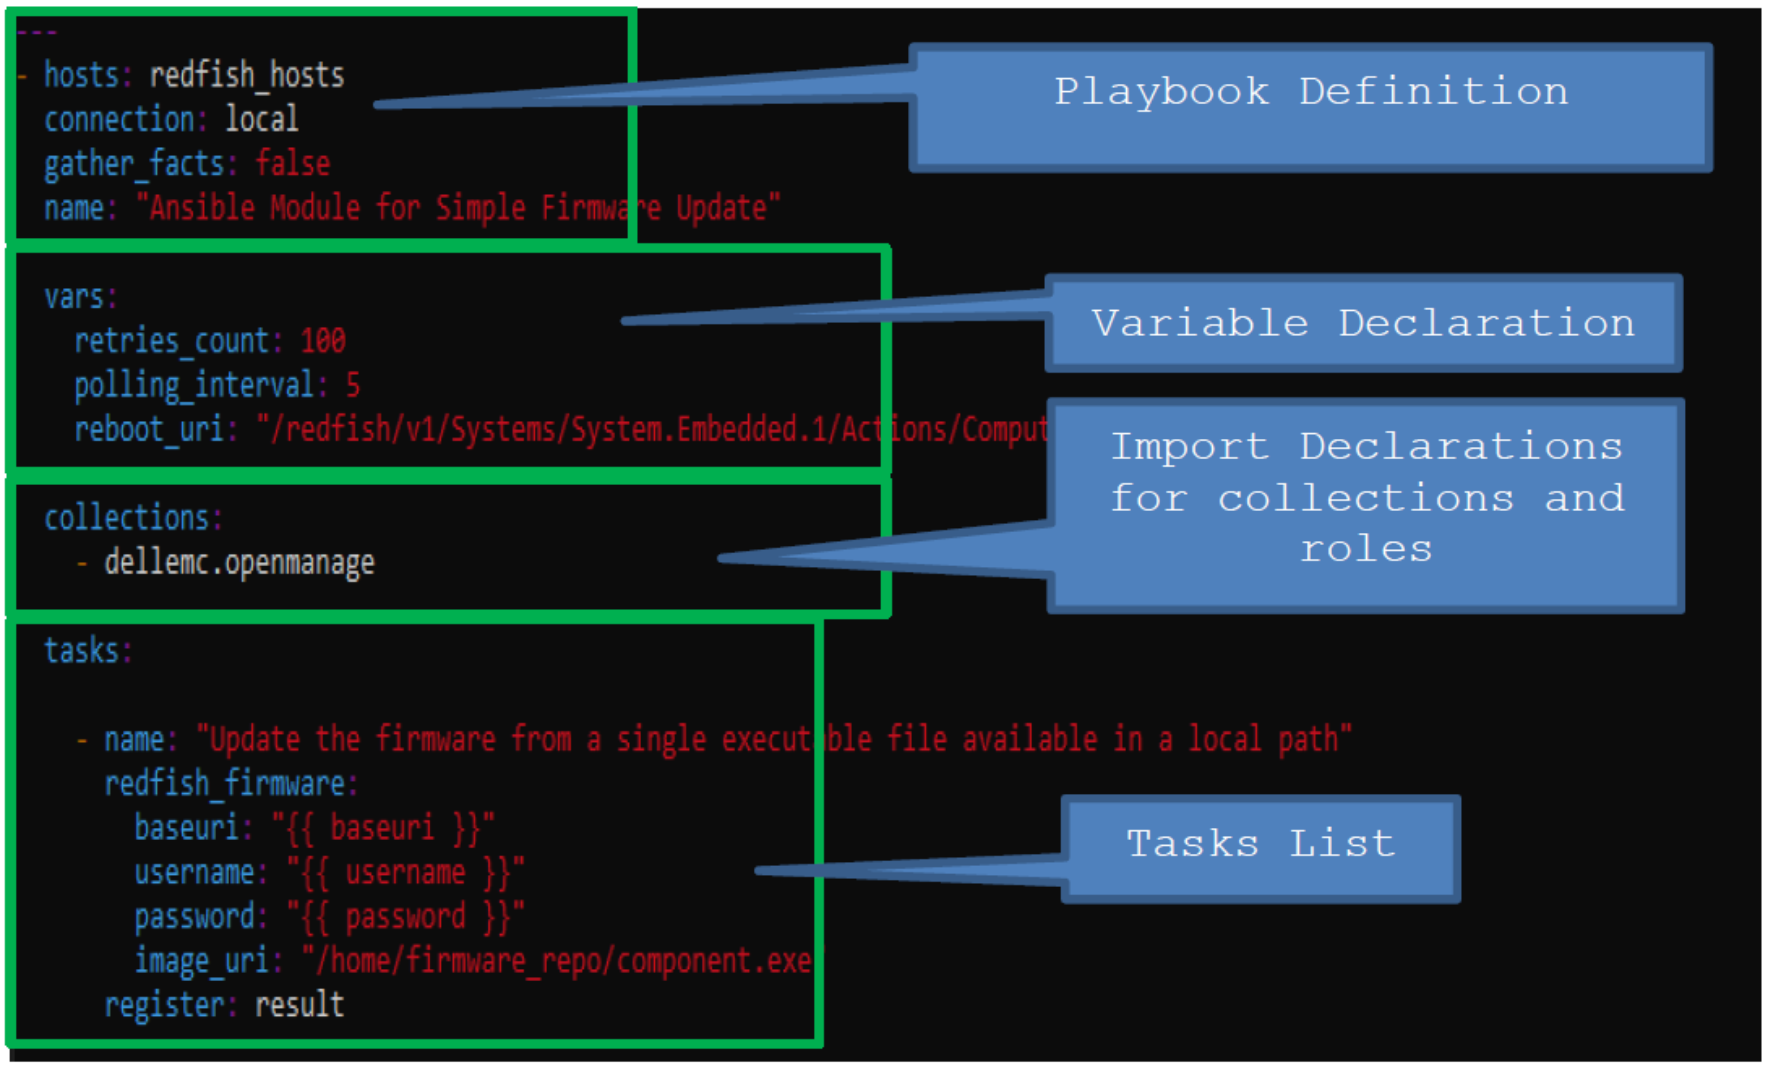
\includegraphics[scale=0.9]{playbook.png}
  \end{center}
  \caption[การเขียนไฟล์ playbook]{การเขียนไฟล์ playbook}
  \label{fig:ansible_playbook}
\end{figure}

\subsection{Modules}
\hspace{0.5in} โมดูล python ที่ใช้เพื่อดำเนินการจัดการ tasks ต่างๆบนระบบปลายทาง
\subsection{Roles}
\hspace{0.5in} กลุ่มของ tasks ที่สามารถ reuse ได้

\section{Ansible AWX}
\hspace{0.5in} Ansible AWX เป็นเว็บอินเตอร์เฟสสำหรับ Ansible ช่วยให้ผู้ใช้สามารถจัดการ Ansible playbooks และ inventories ผ่านเว็บเบราว์เซอร์โดยไม่ต้องพึ่ง command line ทำให้การจัดการโครงสร้างพื้นฐาน IT ด้วย Ansible นั้นง่ายขึ้นและสะดวกยิ่งขึ้น 
อีกทั้งยังมี API ที่สามารถนำมาใช้พัฒนาเพิ่มเติมได้

\begin{figure}[h]
  \begin{center}
    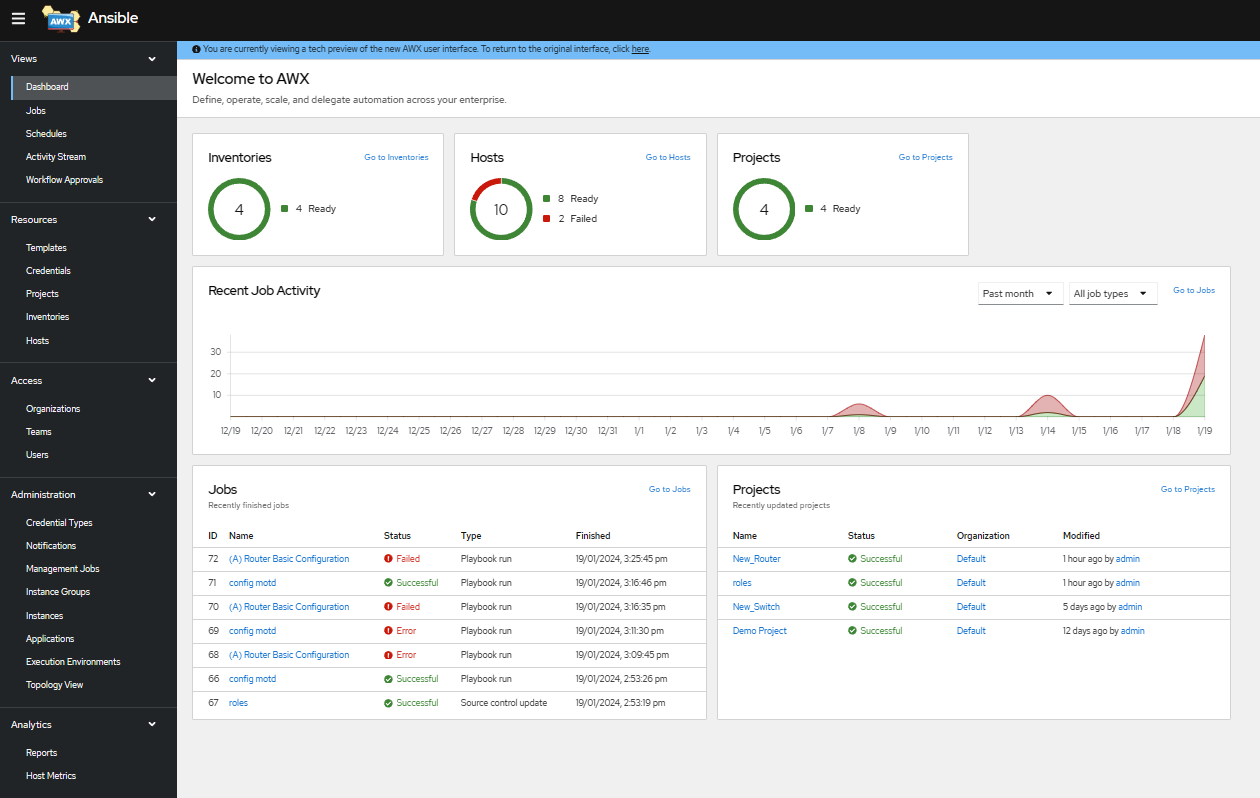
\includegraphics[scale=0.55]{awx.png}
  \end{center}
  \caption[ตัวอย่างการแสดงผลของ Ansible AWX]{ตัวอย่างการแสดงผลของ Ansible AWX}
  \label{fig:ansible_playbook}
\end{figure}

\hspace{0.3in} โดยส่วนสำคัญของ Ansible AWX ได้แก่


\subsection{Dashboard}
\hspace{0.5in} แสดงสถานะทั้งหมดของ Ansible AWX และการทำงานของ Ansible เอาไว้โดยรวม เช่น จำนวน hosts จำนวน project หรือสถานะของงานที่เคยเรียกใช้ ว่าสำเร็จหรือไม่สำเร็จ

\subsection{Inventory}
\hspace{0.5in} ใช้สำหรับจัดกลุ่มเพื่อรวบรวม และจัดการ hosts ต่างๆ ที่จะต้องใช้งานเอาไว้ โดยสามารถเพิ่มหรือจัดการ hosts เหล่านั้นเองได้

\subsection{Projects}
\hspace{0.5in} ใช้จัดการโค้ดของ Ansible ที่จะใช้งาน ซึ่งคล้ายกับ git โดยจะเก็บ playbook เก็บ inventory และตัวแปรต่างๆที่เกี่ยวข้องเอาไว้

\subsection{Hosts}
\hspace{0.5in} แสดงรายการ host ต่างๆที่เอาไว้ใช้งาน โดย hosts เหล่านี้จะถูกจัดเก็บอยู่ใน inventory ซึ่งจะแสดงว่า host แต่ละตัวนั้นถูกเก็บโดย inventory ไหนบ้าง

\subsection{Credentials}
\hspace{0.5in} ใช้สำหรับยืนยันตัวตนเช่น ชื่อผู้ใช้ รหัสผ่าน คีย์ ssh หรือข้อมูลอื่นๆที่ ansible ต้องการ

\subsection{Templates}
\hspace{0.5in} ใช้สร้างงานต่างๆ โดยจะทำงานร่วมกับ playbook และ inventory ที่เราสร้างไว้ ซึ่งเราสามารถรวม งานหลายๆงานให้ทำงานต่อเนื่องกันไว้ใน template เดียว ผ่าน workflow template

\subsection{Jobs}
\hspace{0.5in} แสดงผลลัพธ์และสถานะของงานนั้นๆที่เคยถูกเรียกใช้ทั้งหมด ว่าสำเร็จหรือไม่สำเร็จ หรือมี error เกิดขึ้น

\section{\ifenglish%
\ifcpe CPE \else ISNE \fi knowledge used, applied, or integrated in this project
\else%
ความรู้ตามหลักสูตรซึ่งถูกนำมาใช้หรือบูรณาการในโครงงาน
\fi
}
\begin{enumerate}
\item การเข้าใช้เครือข่าย การจัดการระบบเครือข่ายและความรู้ด้านเครือข่ายจากวิชา เครือข่ายคอมพิวเตอร์ (Computer Network 261335) 
\item ชุดคำสั่งการตั้งค่าของระบบเครือข่าย การดูแลระบบเน็ตเวิร์คและการตรวจสอบชุดคำสั่งทางด้านเครือข่ายจากวิชา ปฏิบัติการเครือข่ายคอมพิวเตอร์ (Computer Network Laboratory 261336)
\item กระบวนการพัฒนาโปรแกรมจากวิชาวิศวกรรมซอฟต์แวร์ (Software Engineer 261361)
\end{enumerate}

\section{\ifenglish%
Extracurricular knowledge used, applied, or integrated in this project
\else%
ความรู้นอกหลักสูตรซึ่งถูกนำมาใช้หรือบูรณาการในโครงงาน
\fi
}

\begin{enumerate}
  \item การทำงานของ Ansible
  \item การทำงานและวิธีใช้งาน Ansible AWX
\end{enumerate}

\chapter{\ifproject%
\ifenglish Project Structure and Methodology\else โครงสร้างและขั้นตอนการทำงาน\fi
\else%
\ifenglish Project Structure\else โครงสร้างของโครงงาน\fi
\fi
}

\makeatletter

% \renewcommand\section{\@startsection {section}{1}{\z@}%
%                                    {13.5ex \@plus -1ex \@minus -.2ex}%
%                                    {2.3ex \@plus.2ex}%
%                                    {\normalfont\large\bfseries}}

\makeatother
%\vspace{2ex}
% \titleformat{\section}{\normalfont\bfseries}{\thesection}{1em}{}
% \titlespacing*{\section}{0pt}{10ex}{0pt}

\section{การออกแบบ}

\subsection{Ansible}
\hspace{0.5in} Ansible เป็น Open Source Software Automation Tool ที่ใช้ YAML syntax ในการเขียน Playbook เพื่อทำการตั้งค่าอุปกรณ์เครือข่าย ข้อดีของการใช้ Ansible ในการออกแบบมีดังนี้ 
\begin{itemize}
  \item ใช้งานง่าย: Ansible เขียนด้วย YAML syntax เข้าใจง่าย
  \item Agentless: ไม่จำเป็นต้องติดตั้ง agent บนเครื่อง Remote
  \item Powerful: รองรับการ Automation งานต่างๆ มากมาย
  \item Flexible: รองรับระบบปฏิบัติการหลายประเภท
\end{itemize}
\hspace{0.5in} แต่การใช้งานเพียงแค่ Ansible สำหรับการตั้งค่าเครือข่ายนั้นมีความค่อนข้างยุ่งยากเนื่องจากต้องทำงานผ่าน CLIs ซึ่งอาจเป็นเรื่องยากสำหรับผู้ใช้บางคน

\subsection{AWX}
\hspace{0.5in} AWX เป็น Open Source Web Application ที่ช่วยจัดการ Workflow ของ Ansible โดยสั่งผ่าน GUI ดังนั้นโครงงานนี้จึงเลือกที่จะใช้ AWX เป็น GUI สำหรับควบตุมการทำงานของ Ansible ซึ่งข้อดีของการใช้ AWX ในการจัดการอุปกรณ์เครือข่าย มีดังนี้
\begin{itemize}
  \item Centralized Management: ควบคุมจัดการ Jobs, Playbooks, Inventory และ Credentials ทั้งหมดจากจุดเดียว
  \item Role-Based Access Control: กำหนดสิทธิ์การเข้าถึงสำหรับผู้ใช้แต่ละคน
  \item Integrations: รองรับการผสานรวมกับ Tools อื่นๆ เช่น Jenkins, GitLab และ GitHub
  \item Notification: มีการแจ้งเตือนผู้ใช้เมื่อมี Errors เกิดขึ้น
\end{itemize}
\hspace{0.5in} การใช้ AWX ใน Web Application สำหรับ Automation จะช่วยติดตามสถานะการทำงาน จัดการกลุ่มเป้าหมาย (Inventory) ค้นหาและดูข้อมูลย้อนหลัง และสามารถตรวจสอบปัญหาต่างๆที่เกิดขึ้นในเมื่อเกิด Errors

\subsection{Web Application}
\hspace{0.5in} เนื่องจากการใช้งาน Ansible AWX นั้นมีข้อดีที่สามารถเข้าไปจัดการตั้งค่าอุปกรณ์ได้ทีละหลายอุปกรณ์ แต่ยังมีข้อจำกัดคือ ไม่สามารถเช็คความถูกต้องว่าผู้ใช้งานตั้งค่าอุปกรณ์เครือข่ายจากการรัน Templates บน Ansible AWX แล้วอุปกรณ์เครือข่ายนั้นทำงานได้ถูกต้องจริงหรือไม่ จึงทำการออกแบบ Web Application ที่มีระบบตรวจสอบความถูกต้อง และสามารถใช้ AWX REST API ในการดึงข้อมูลของอุปกรณ์เครือข่ายทำที่ได้ทำการตั้งค่าไว้ มาแสดงใน Web Application และสามารถนำคำสั่งที่เขียนใน Ansible Playbooks มาตรวจสอบความถูกต้องว่าคำสั่งที่สั่ง ครบหรือไม่ หรือ เช็คว่าการทำงานของอุปกรณ์ เน็ตเวิร์คทำงานถูกต้องหรือไม่

\section{โครงสร้างการทำงาน}
\hspace{0.5in} การทำงานของ Web Application จะเป็นการใช้ AWX API มาแสดงผลบน Web Application ที่สร้างขึ้นมาโดยจะมีฟังก์ชันหลักๆดังนี้
\begin{itemize}
  \item Configuration: โดยผู้ใช้จะไม่ต้องสร้าง Templates ขึ้นมาเองเนื่องจาก Templates นั้นถูกสร้างแบบสำเร็จรูปไว้เรียบร้อยแล้วใน Ansible AWX โดยผู้ใช้จะทำเพียงแค่เลือก Templates ที่ผู้ใช้ต้องการจัดการและกรอกข้อมูล Hosts และ Configuration ต่างๆใน Web Application จากนั้น Web Application จะนำข้อมูลที่ผู้ใช้กรอกส่งไปยัง Ansible AWX เพื่อให้ Ansible AWX รับคำสั่งและทำตามคำสั่งเหล่านั้นในอุปกรณ์เน็ตเวิร์คที่ผู้ใช้ได้กำหนดไว้
  \item Verification: 
\end{itemize}
\chapter{\ifproject%
\ifenglish Experimentation and Results\else ประเมินระบบ\fi
\else%
\ifenglish System Evaluation\else การประเมินระบบ\fi
\fi}

\hspace{0.5in} การประเมินระบบโครงงาน เพื่อวัดความสามารถและประสิทธิภาพของระบบว่าระบบของโครงงานนี้สามารถทำงานได้ถูกต้องและมีประสิทธิภาพ แบ่งออกเป็น 3 ส่วนดังนี้

\section{อุปกรณ์เครือข่ายทำงานได้ถูกต้องตามที่ผู้ใช้ได้ทำการตั้งค่าผ่าน Web Application}
เมื่อผู้ใช้ทำการตั้งค่าอุปกรณ์เครือข่ายโดยทำผ่าน UI ของ Web application อุปกรณ์เครือข่ายที่ถูกตั้งค่านั้นจะต้องมีค่าการตั้งค่าที่เหมือนกับที่ผู้ใช้ได้ระบุผ่าน Web Application 
\section{Web Application มีระบบที่สามารถดึงข้อมูลการตั้งค่าจากอุปกรณ์เครือข่ายที่ถูกต้อง}
เมื่อต้องทำการตรวจสอบความถูกต้องของการทำงานอุปกรณ์เครือข่าย ระบบจะต้องสามารถดึงข้อมูลการตั้งค่าจากอุปกรณ์เครือข่ายแต่ละตัวและข้อมูลที่ดึงมานั้นต้องมีค่าที่ตรงกับค่าการตั้งค่าของอุปกรณ์เครือข่ายที่มีอยู่ภายในอุปกรณ์
\section{โปรแกรมมีระบบตรวจสอบการทำงานอุปกรณ์เครือข่ายที่ถูกต้อง}
หลังจากที่ได้ข้อมูลการตั้งค่าของอุปกรณ์เครือข่าย ระบบจะต้องสามารถคำนวณและบอกได้ว่าการตั้งค่าของอุปกรณ์เครือข่ายเครื่องนั้นสามารถทำงานได้ถูกต้อง

\ifproject
\chapter{\ifenglish Conclusions and Discussions\else บทสรุปและข้อเสนอแนะ\fi}

\section{\ifenglish Conclusions\else สรุปผล\fi}

\hspace{0.5in}โครงงานนี้ได้จัดทำแอพพลิเคชั่นตั้งค่าและตรวจสอบอุปกรณ์เครือข่ายอัตโนมัติโดยใช้แอนสิเบิล
สำหรับบุคคลทั่วไป หรือผู้ดูแลระบบที่ไม่ชำนาญการใช้ชุดคำสั่งแบบ CLIs โดยใช้ Ansible AWX เพื่อ
รับข้อมูลและสั่งการให้อุปกรณ์เครือข่ายทำงานตามที่ต้องการ จากการทดสอบระบบพบว่า

\section{\ifenglish Challenges\else ปัญหาที่พบและแนวทางการแก้ไข\fi}

\hspace{0.5in}ในการทำโครงงานนี้ พบว่าเกิดปัญหาหลักๆ ดังนี้
\begin{enumerate}
    \item การเรียกใช้งาน Templates ที่ต้องเรียกใช้งานผ่าน online เท่านั้น
    \item อะไรอีก
  \end{enumerate}
\section{\ifenglish%
Suggestions and further improvements
\else%
ข้อเสนอแนะและแนวทางการพัฒนาต่อ
\fi
}

\hspace{0.5in}ข้อเสนอแนะเพื่อพัฒนาโครงงานนี้ต่อไป มีดังนี้
\begin{enumerate}
    \item อ่าา
    \item อะไรอีก
  \end{enumerate}

\fi

\bibliography{sampleReport}

\ifproject
\normalspacing
\appendix
\chapter{The first appendix}

Text for the first appendix goes here.

\section{Appendix section}

Text for a section in the first appendix goes here. 

test ทดสอบฟอนต์ serif ภาษาไทย aasdasdasd 

\textsf{test ทดสอบฟอนต์ sans serif ภาษาไทย}

\verb+test ทดสอบฟอนต์ teletype ภาษาไทย+

\texttt{test ทดสอบฟอนต์ teletype ภาษาไทย}

\textbf{ตัวหนา serif ภาษาไทย \textsf{sans serif ภาษาไทย} \texttt{teletype ภาษาไทย}}

\textit{ตัวเอียง serif ภาษาไทย \textsf{sans serif ภาษาไทย} \texttt{teletype ภาษาไทย}}

\textbf{\textit{ตัวหนาเอียง serif ภาษาไทย \textsf{sans serif ภาษาไทย} \texttt{teletype ภาษาไทย}}}

\url{https://www.example.com/test_ทดสอบ_url}

\chapter{\ifenglish Manual\else คู่มือการใช้งานระบบ\fi}

Manual goes here.


%% Display glossary (optional) -- need glossary option.
\ifglossary\glossarypage\fi

%% Display index (optional) -- need idx option.
\ifindex\indexpage\fi

\begin{biosketch}
  \begin{center}
    \includegraphics[width=1.5in]{mugshot.jpg}
  \end{center}
  \hspace{0.5in}ว่านนนนนนนนนนนนนนนนนนนนนนนนนนนนนนนน
\begin{center}
  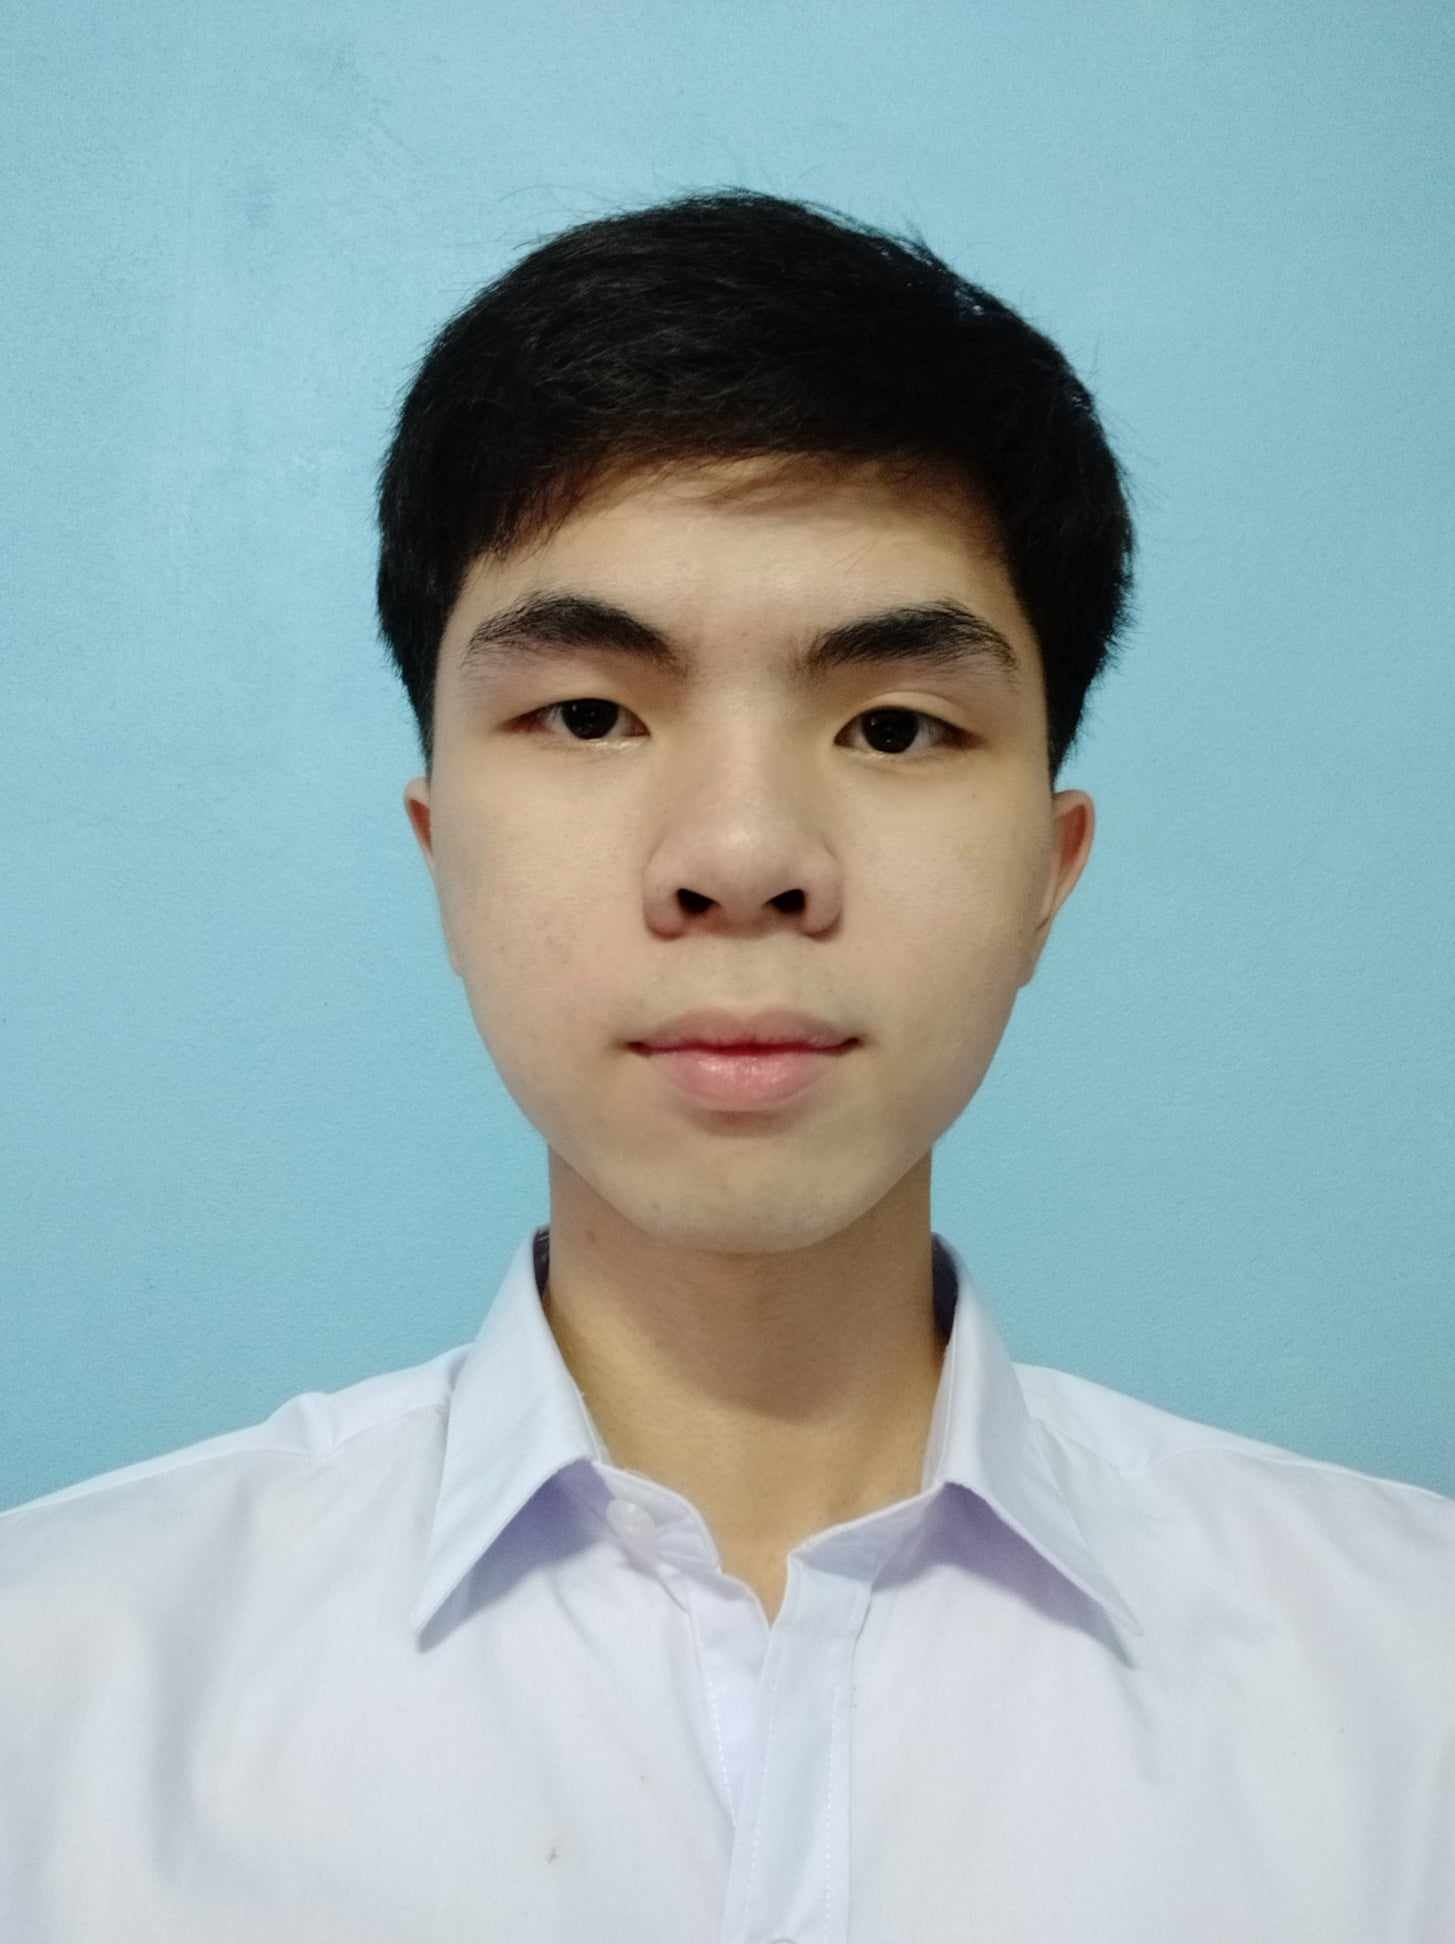
\includegraphics[width=1.5in]{636.jpg}
\end{center}
\hspace{0.5in}นายทัตพงศ์ เสริมสุข เกิดเมื่อวันที่ 13 กันยายน 2545 ณ จังหวัดลำปาง สำเร็จการศึกษาระดับมัธยมศึกษาจากโรงเรียนบุญวาทย์วิทยาลัย เข้าศึกษาที่ภาควิชาวิศวกรรมคอมพิวเตอร์ 
มหาวิทยาลัยเชียงใหม่ เมื่อ มิถุนายน 2564 โดยมีความสนใจเป็นพิเศษในด้าน เครือข่ายคอมพิวเตอร์
\begin{center}
  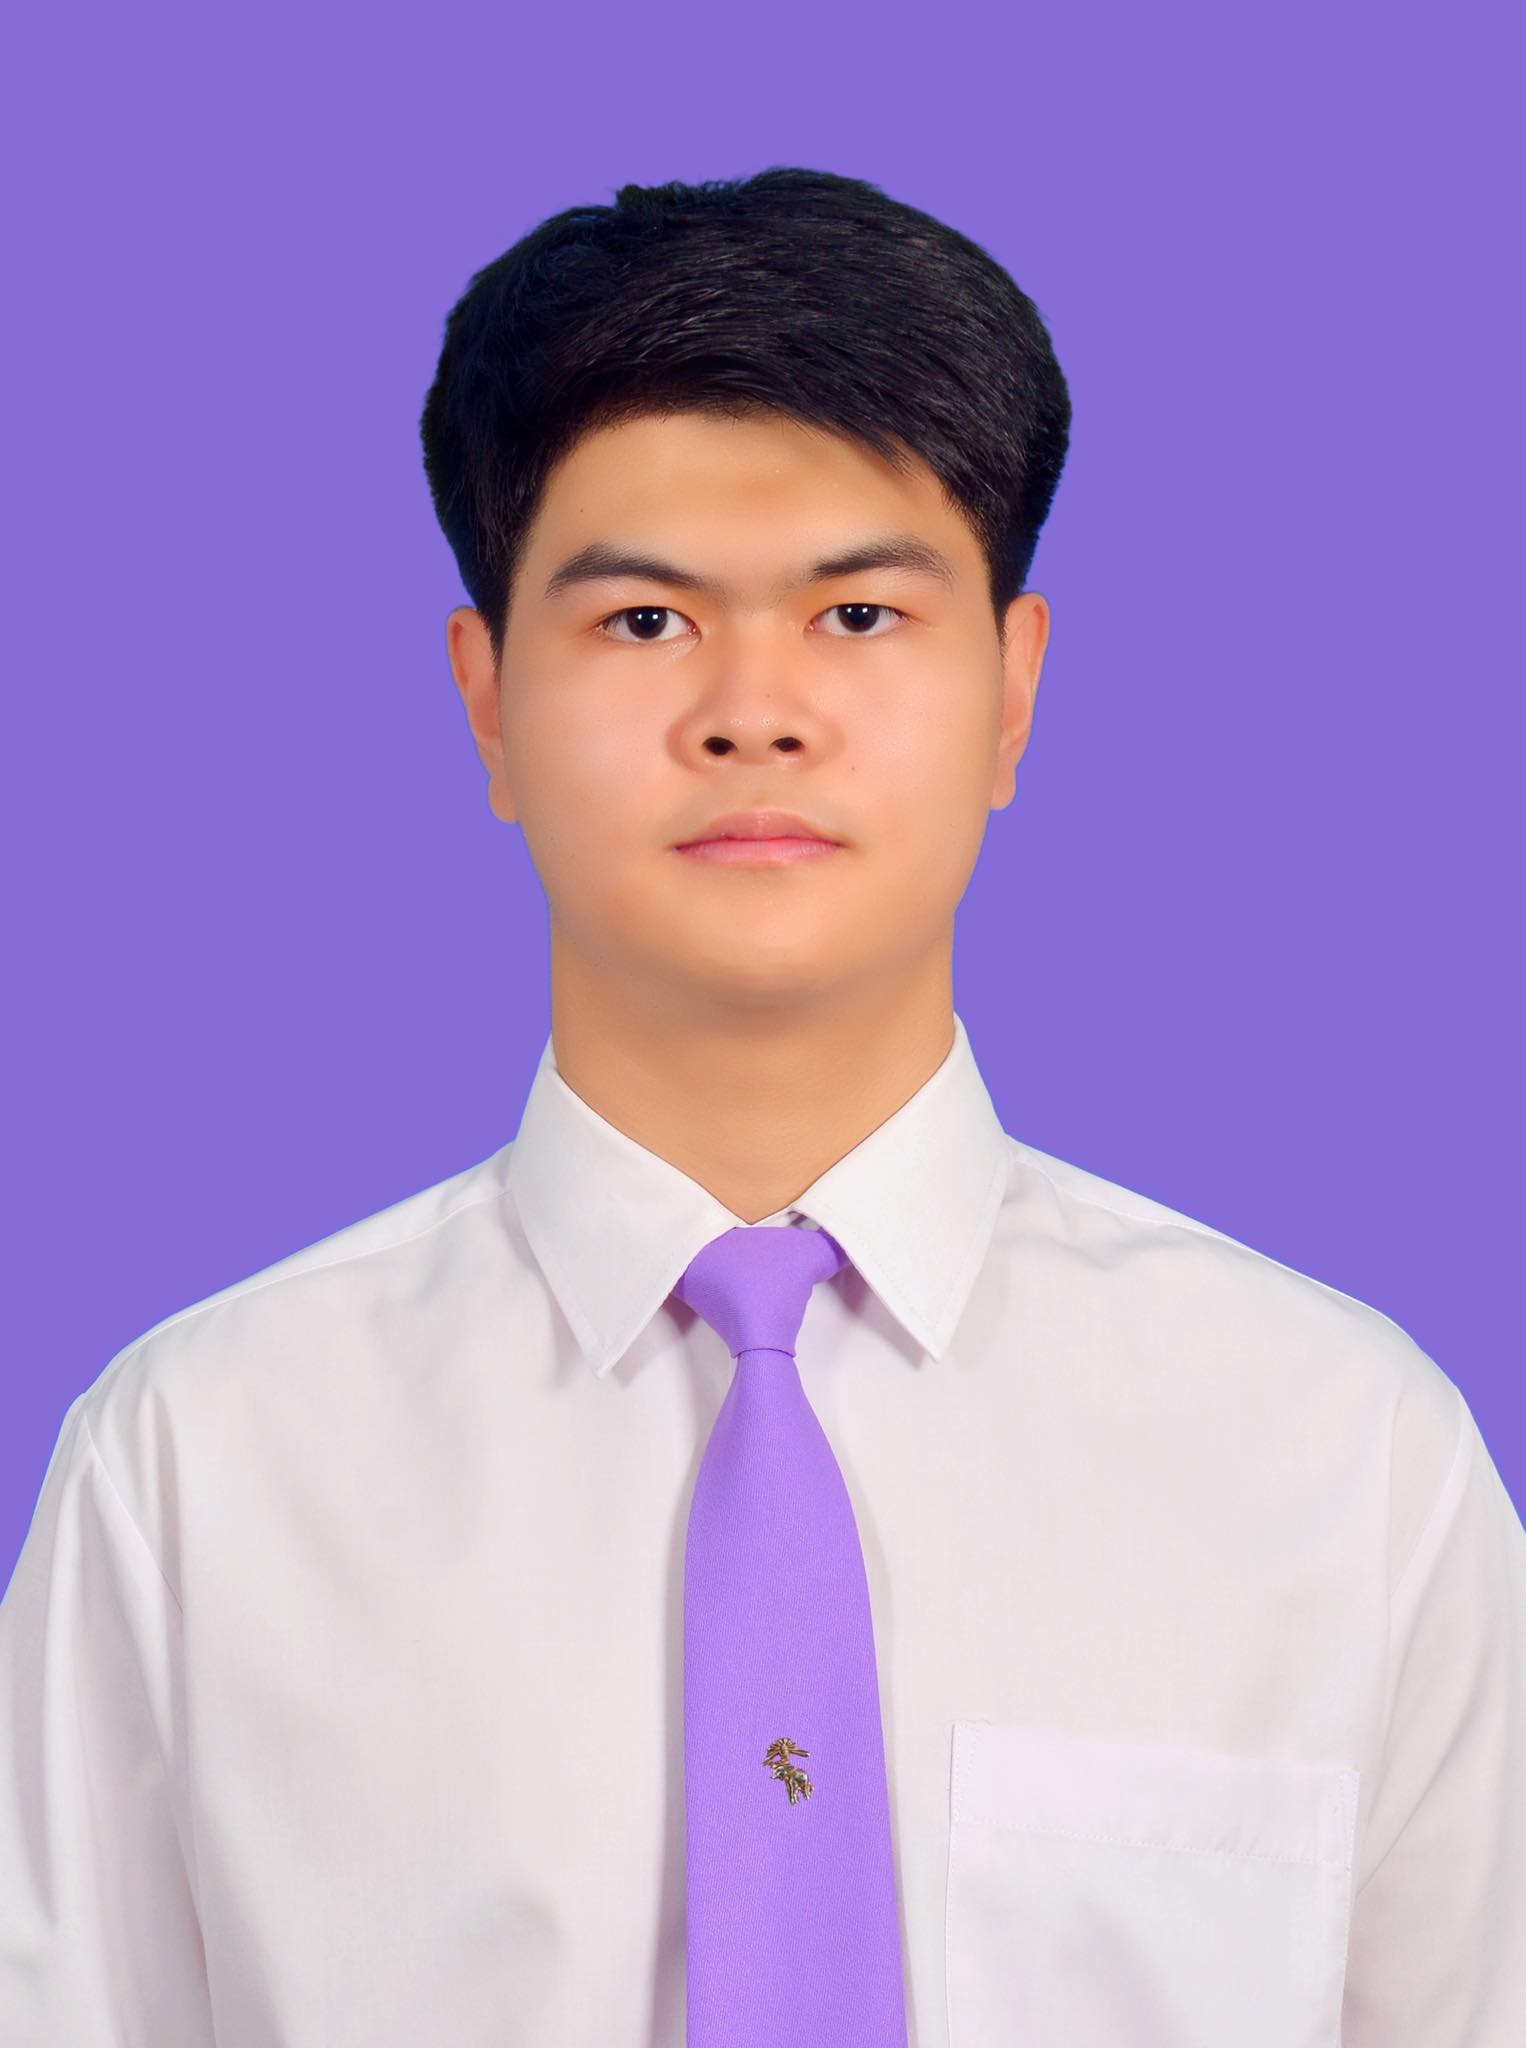
\includegraphics[width=1.5in]{098.jpg}
\end{center}
\hspace{0.5in}นายศุภณัฐ วังทิพย์ เกิดเมื่อวันที่  ณ จังหวัดลำปาง สำเร็จการศึกษาระดับมัธยมศึกษาจากโรงเรียนบุญวาทย์วิทยาลัย เข้าศึกษาที่ภาควิชาวิศวกรรมคอมพิวเตอร์ 
มหาวิทยาลัยเชียงใหม่ เมื่อ มิถุนายน 2564 โดยมีความสนใจเป็นพิเศษในด้าน เครือข่ายคอมพิวเตอร์
\end{biosketch}
\fi % \ifproject
\end{document}

